\begin{figure}[H]
\centering

\includegraphics[width=\textwidth]{7d50bfc38e301fedd7b1324e0990d211.jpg}
% \caption{}
\label{}
\end{figure}

\section{统计文本中单词的个数}

\begin{figure}[H]
\centering
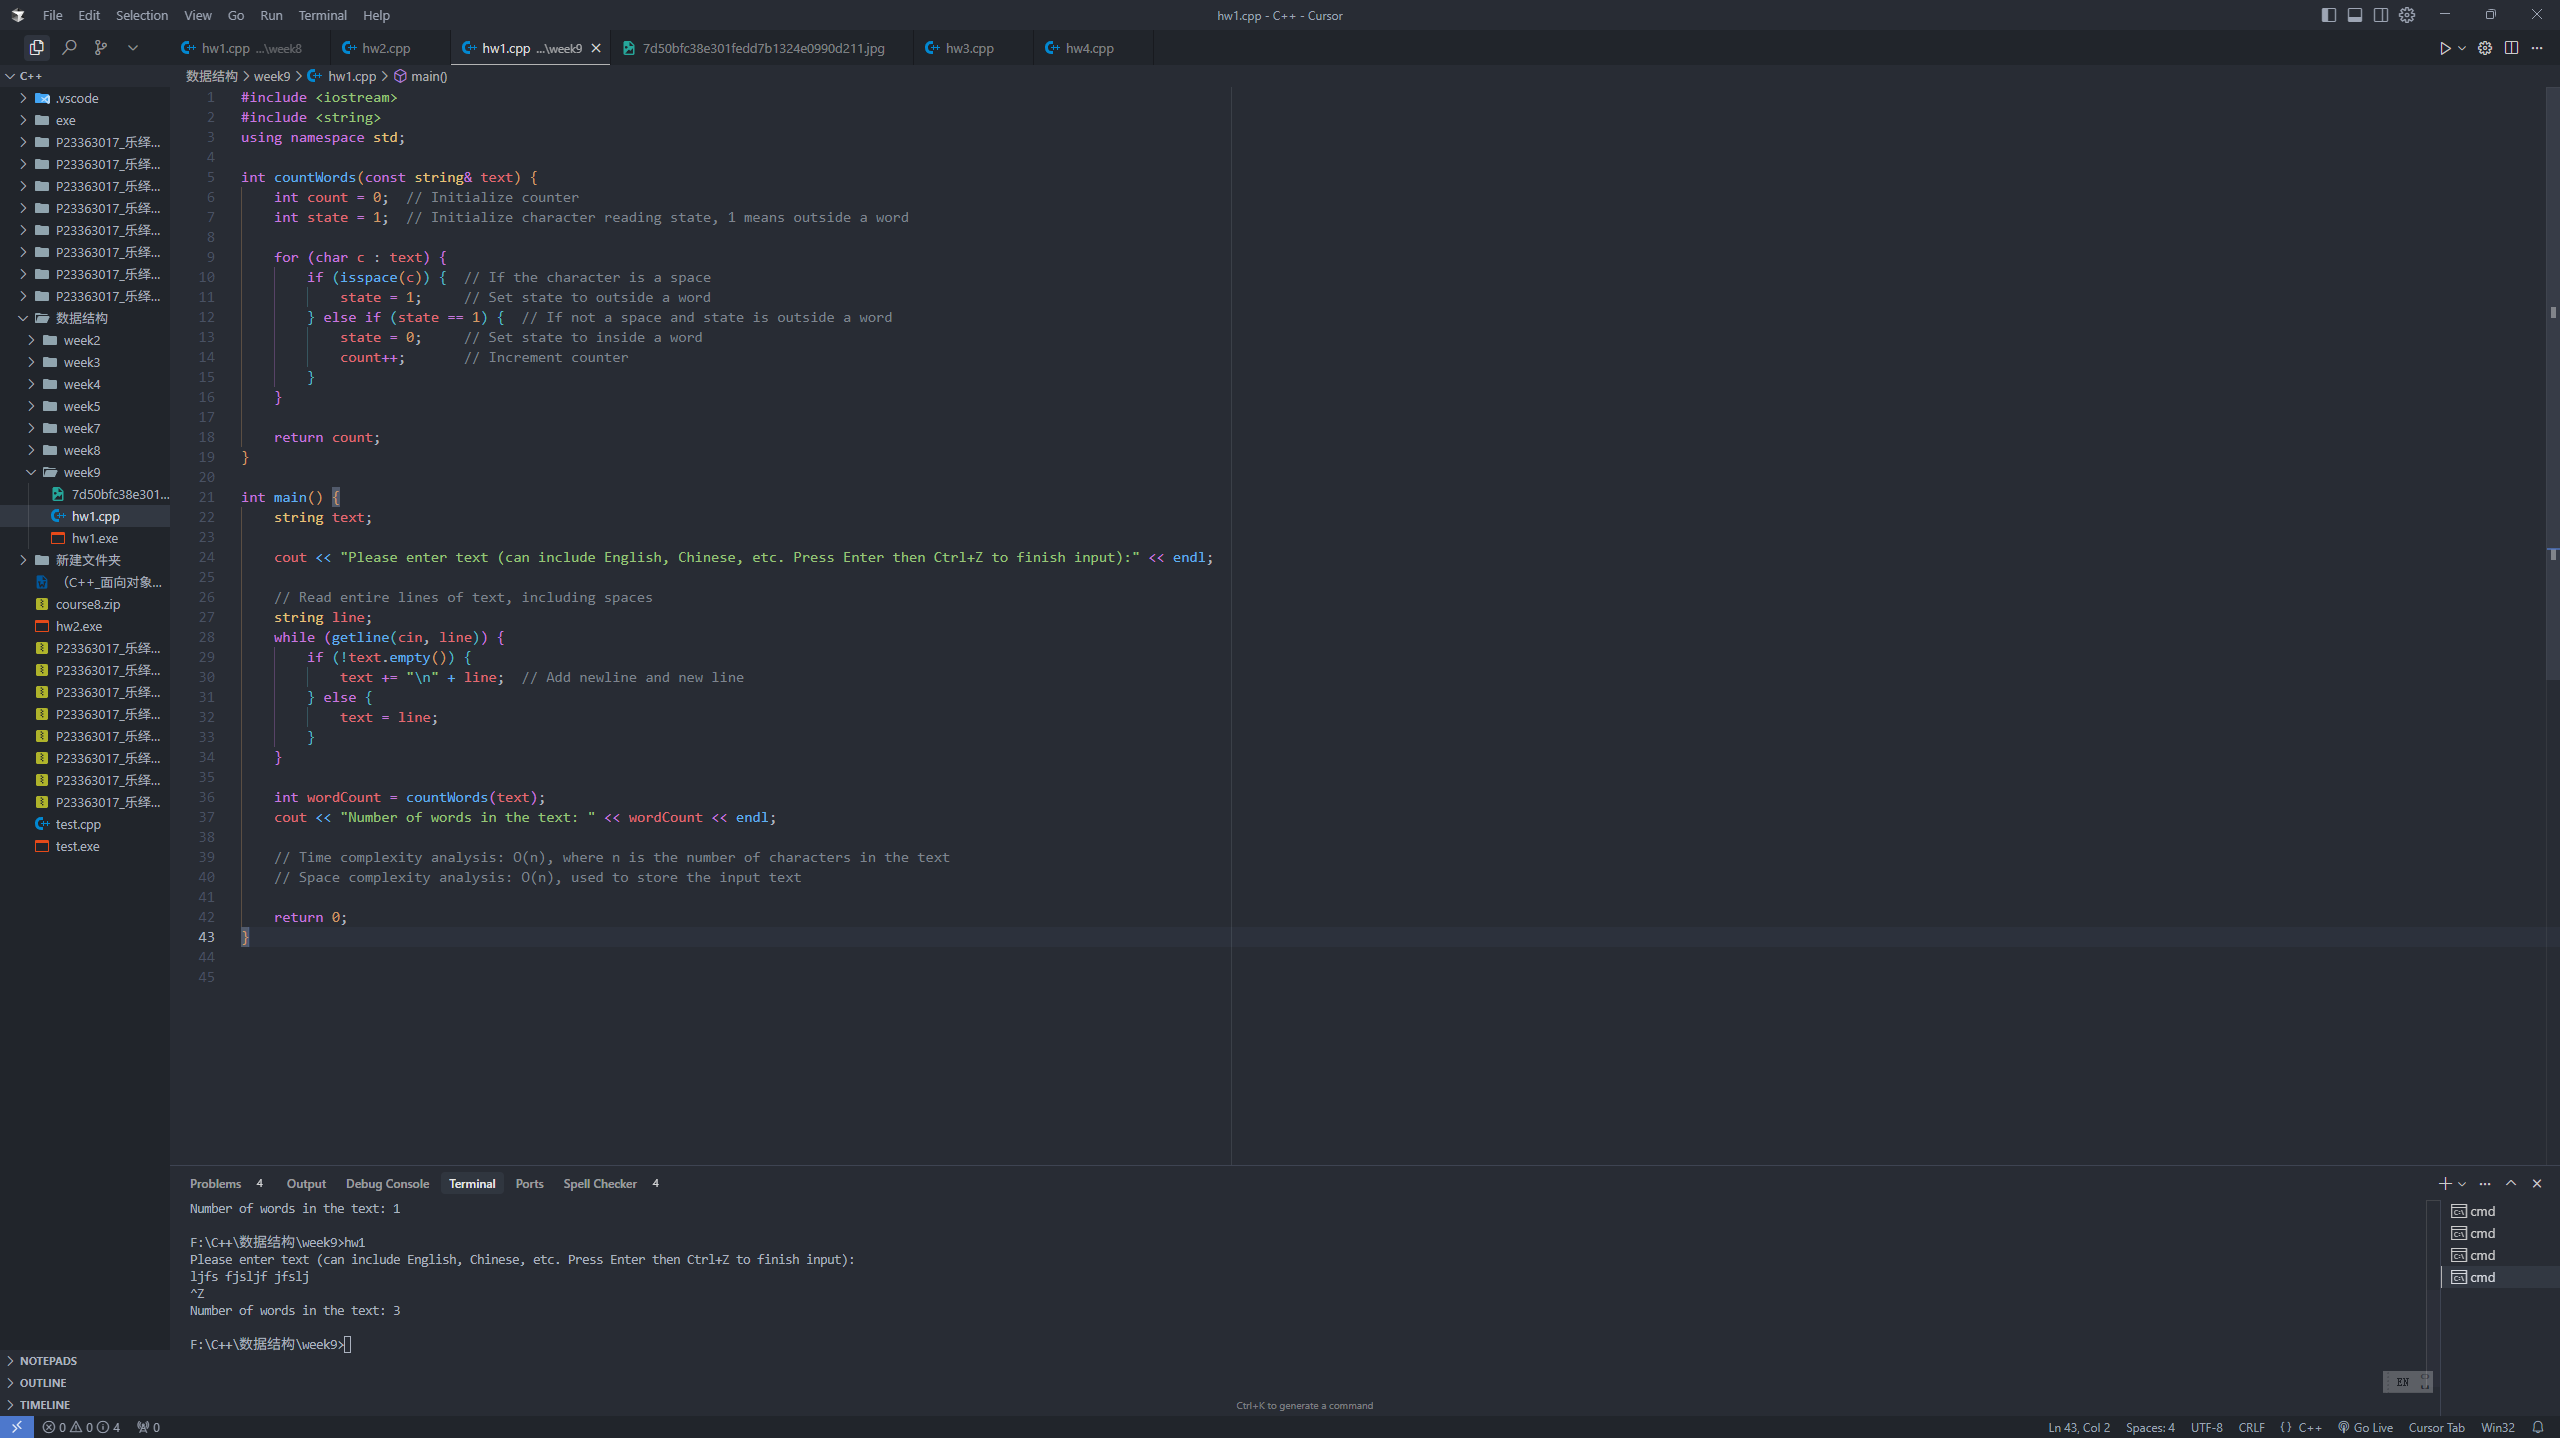
\includegraphics[width=\textwidth]{实验报告8-2025042822.png}
% \caption{}
\label{}
\end{figure}

\begin{lstlisting}[language=C++]
#include <iostream>

#include <string>

using namespace std;

  

int countWords(const string& text) {

    int count = 0;  // Initialize counter

    int state = 1;  // Initialize character reading state, 1 means outside a word

    for (char c : text) {

        if (isspace(c)) {  // If the character is a space

            state = 1;     // Set state to outside a word

        } else if (state == 1) {  // If not a space and state is outside a word

            state = 0;     // Set state to inside a word

            count++;       // Increment counter

        }

    }

    return count;

}

  

int main() {

    string text;

    cout << "Please enter text (can include English, Chinese, etc. Press Enter then Ctrl+Z to finish input):" << endl;

    // Read entire lines of text, including spaces

    string line;

    while (getline(cin, line)) {

        if (!text.empty()) {

            text += "\n" + line;  // Add newline and new line

        } else {

            text = line;

        }

    }

    int wordCount = countWords(text);

    cout << "Number of words in the text: " << wordCount << endl;

    // Time complexity analysis: O(n), where n is the number of characters in the text

    // Space complexity analysis: O(n), used to store the input text

    return 0;

}
\end{lstlisting}
\section{凯撒密码}

\begin{figure}[H]
\centering
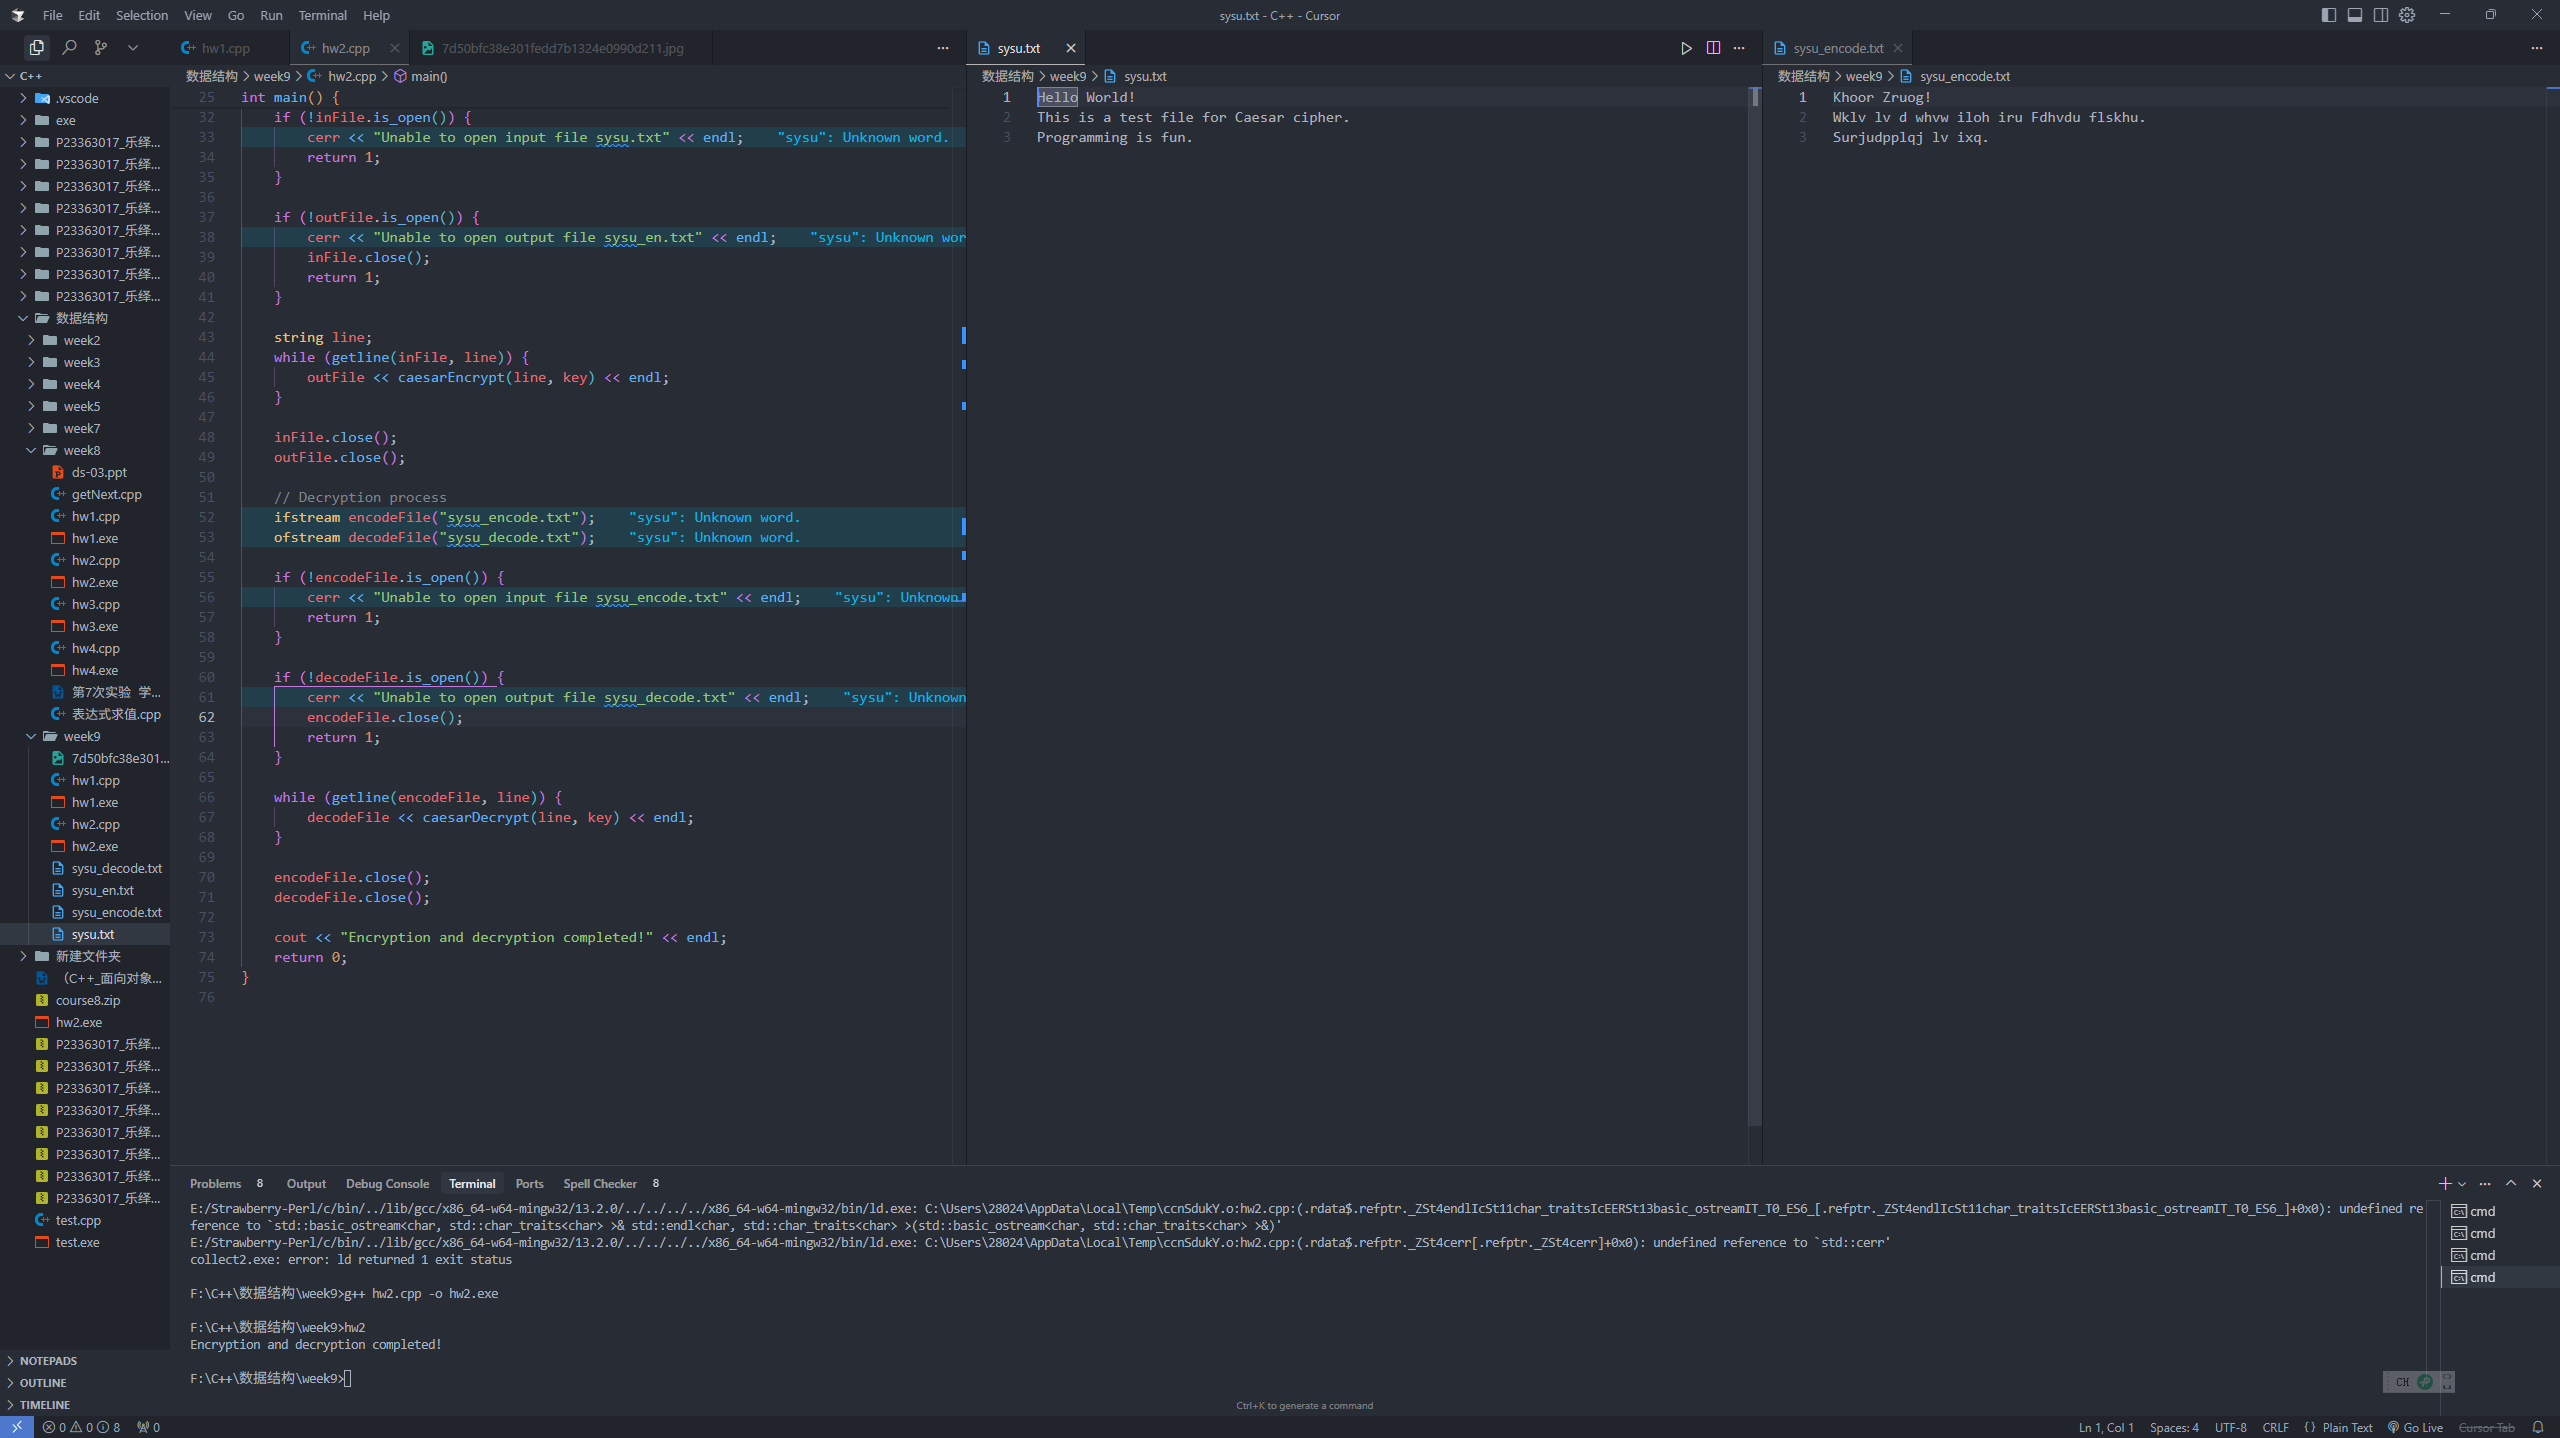
\includegraphics[width=\textwidth]{1-实验报告8-2025042822.png}
% \caption{}
\label{}
\end{figure}

\begin{lstlisting}[language=C++]
#include <iostream>

#include <fstream>

#include <string>

  

using namespace std;

  

// Caesar encryption function

string caesarEncrypt(const string& plaintext, int key) {

    string ciphertext = plaintext;

    for (char& c : ciphertext) {

        if (isalpha(c)) {

            char base = islower(c) ? 'a' : 'A';

            c = base + (c - base + key) % 26;

        }

    }

    return ciphertext;

}

  

// Caesar decryption function

string caesarDecrypt(const string& ciphertext, int key) {

    // Decryption is moving in the opposite direction, equivalent to encrypting with 26-key

    return caesarEncrypt(ciphertext, 26 - key);

}

  

int main() {

    const int key = 3; // Set key to 3 (can be modified as needed)

    // Encryption process

    ifstream inFile("sysu.txt");

    ofstream outFile("sysu_en.txt");

    if (!inFile.is_open()) {

        cerr << "Unable to open input file sysu.txt" << endl;

        return 1;

    }

    if (!outFile.is_open()) {

        cerr << "Unable to open output file sysu_en.txt" << endl;

        inFile.close();

        return 1;

    }

    string line;

    while (getline(inFile, line)) {

        outFile << caesarEncrypt(line, key) << endl;

    }

    inFile.close();

    outFile.close();

    // Decryption process

    ifstream encodeFile("sysu_encode.txt");

    ofstream decodeFile("sysu_decode.txt");

    if (!encodeFile.is_open()) {

        cerr << "Unable to open input file sysu_encode.txt" << endl;

        return 1;

    }

    if (!decodeFile.is_open()) {

        cerr << "Unable to open output file sysu_decode.txt" << endl;

        encodeFile.close();

        return 1;

    }

    while (getline(encodeFile, line)) {

        decodeFile << caesarDecrypt(line, key) << endl;

    }

    encodeFile.close();

    decodeFile.close();

    cout << "Encryption and decryption completed!" << endl;

    return 0;

}
\end{lstlisting}
\section{对称矩阵相乘}

\begin{figure}[H]
\centering
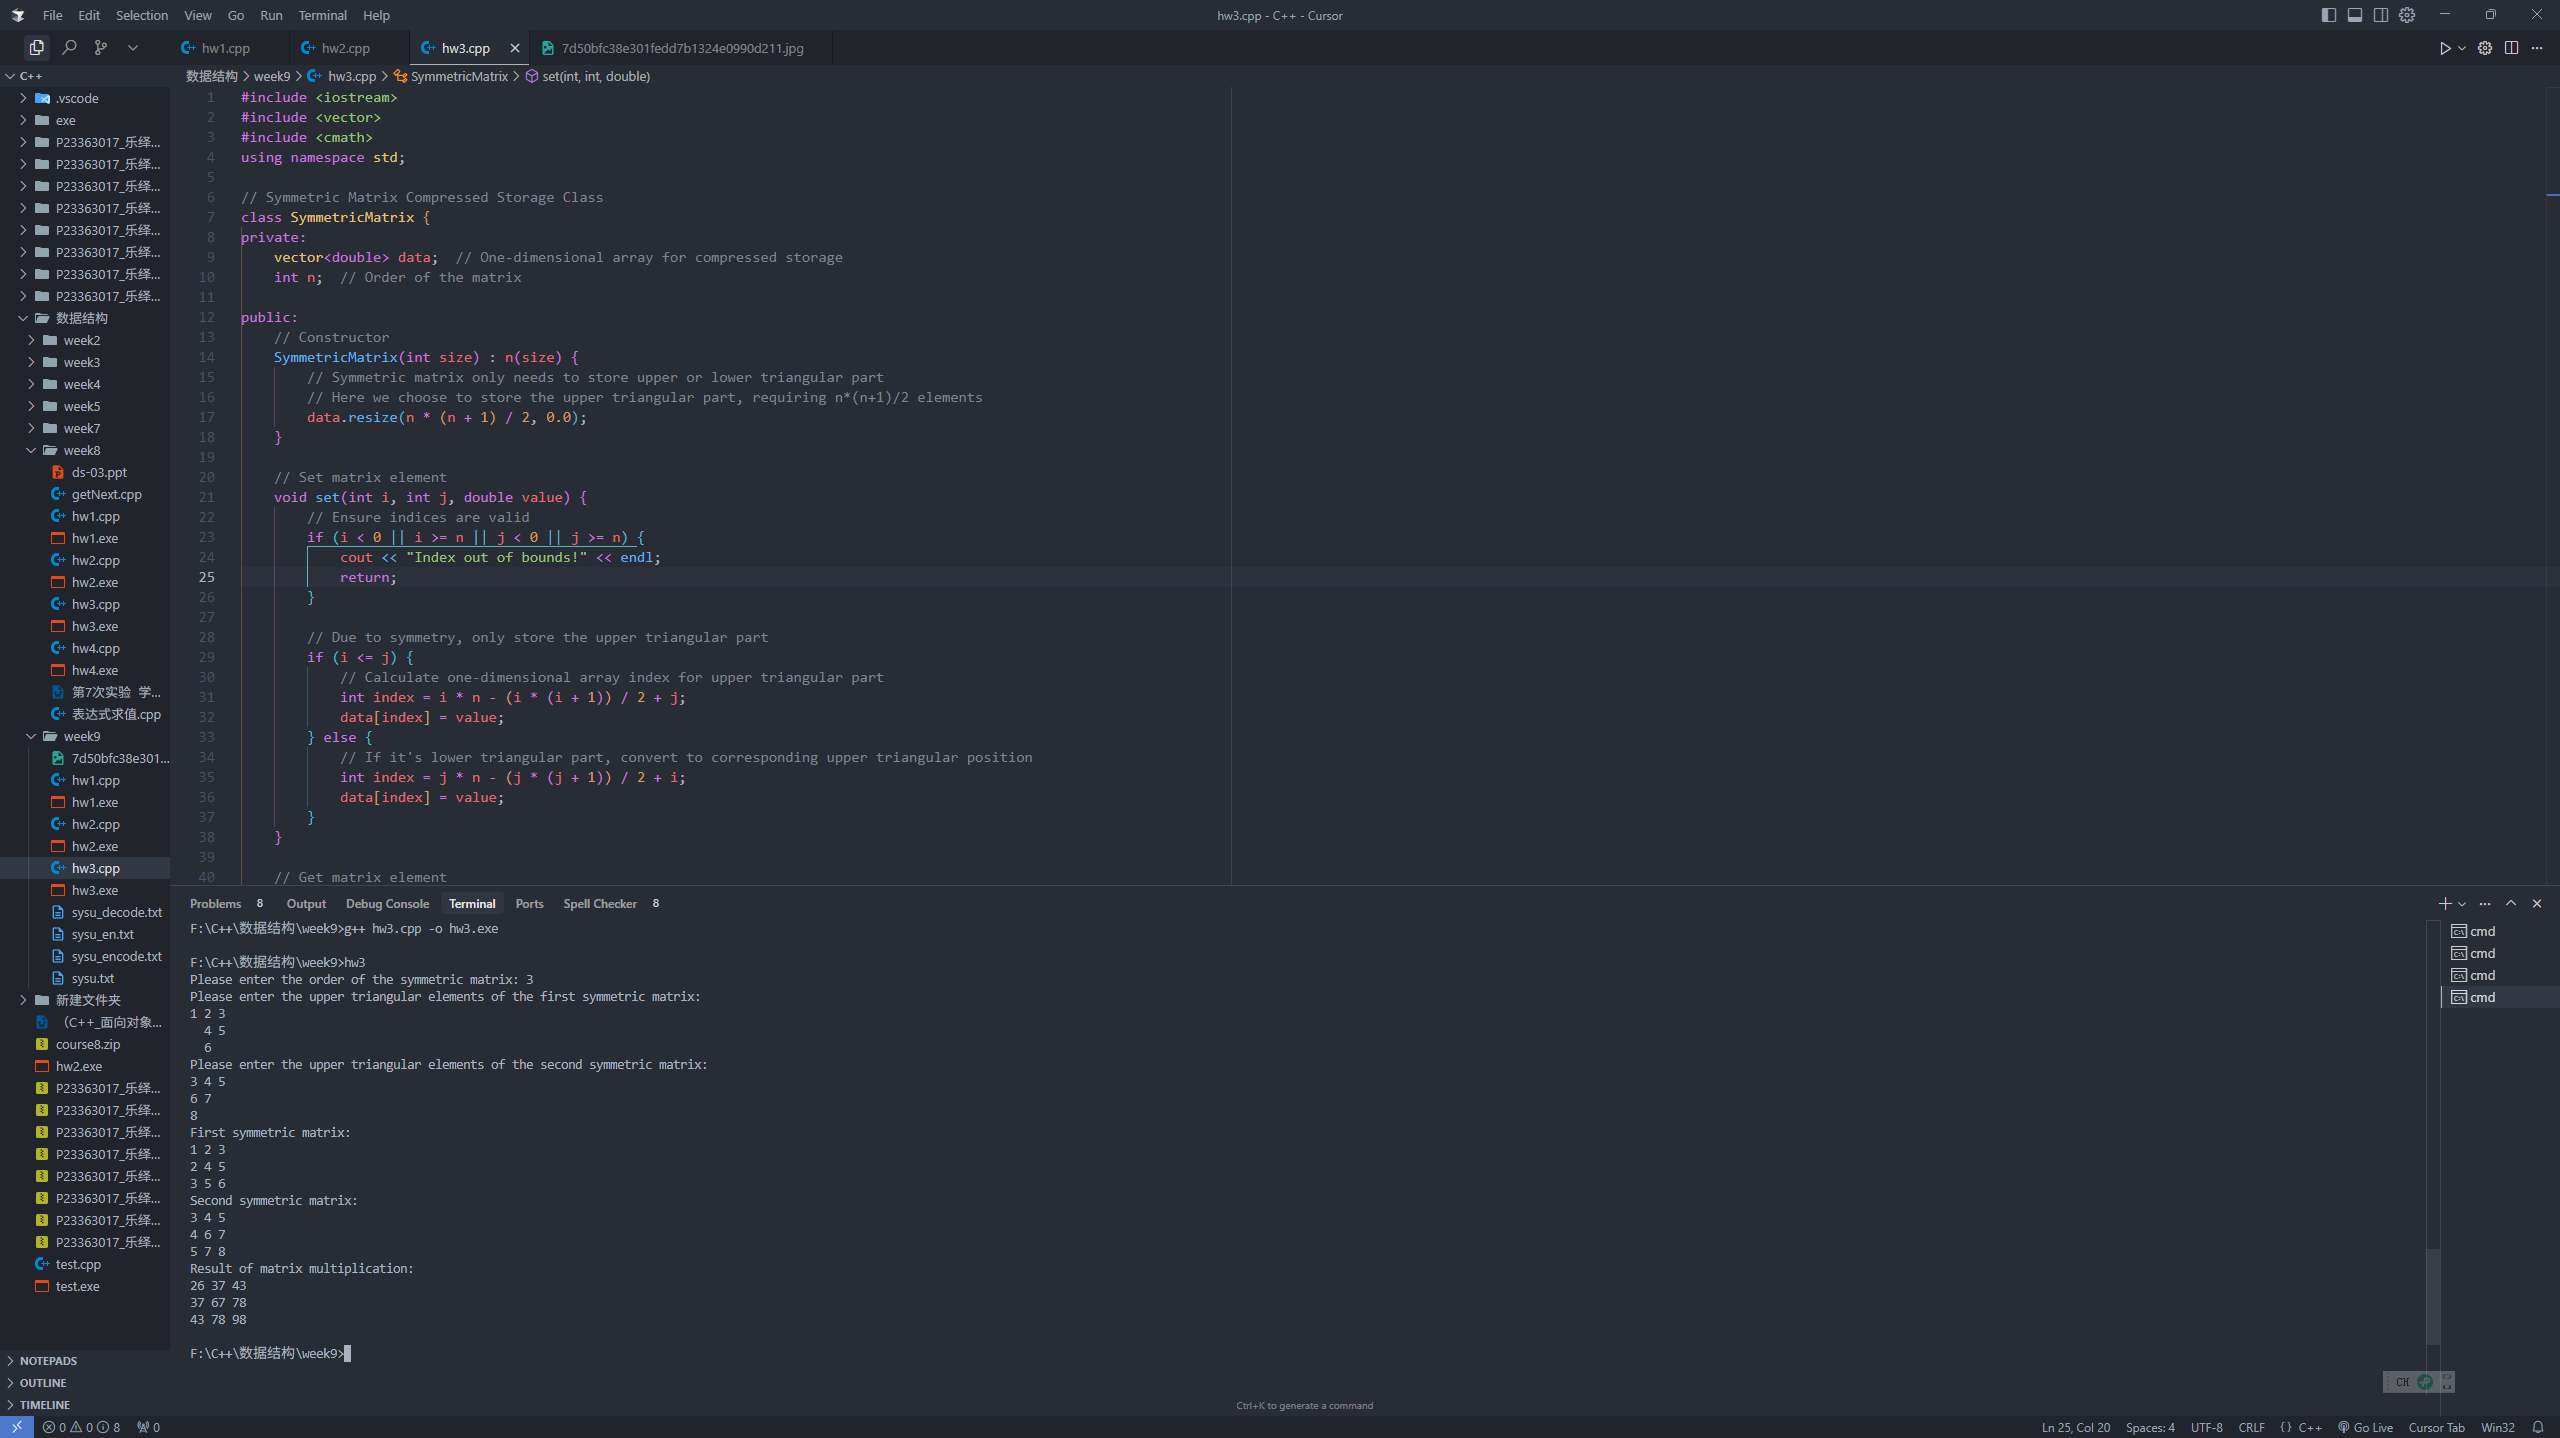
\includegraphics[width=\textwidth]{实验报告8-2025042823.png}
% \caption{}
\label{}
\end{figure}

\begin{lstlisting}[language=C++]
#include <iostream>

#include <vector>

#include <cmath>

using namespace std;

  

// Symmetric Matrix Compressed Storage Class

class SymmetricMatrix {

private:

    vector<double> data;  // One-dimensional array for compressed storage

    int n;  // Order of the matrix

  

public:

    // Constructor

    SymmetricMatrix(int size) : n(size) {

        // Symmetric matrix only needs to store upper or lower triangular part

        // Here we choose to store the upper triangular part, requiring n*(n+1)/2 elements

        data.resize(n * (n + 1) / 2, 0.0);

    }

  

    // Set matrix element

    void set(int i, int j, double value) {

        // Ensure indices are valid

        if (i < 0 || i >= n || j < 0 || j >= n) {

            cout << "Index out of bounds!" << endl;

            return;

        }

        // Due to symmetry, only store the upper triangular part

        if (i <= j) {

            // Calculate one-dimensional array index for upper triangular part

            int index = i * n - (i * (i + 1)) / 2 + j;

            data[index] = value;

        } else {

            // If it's lower triangular part, convert to corresponding upper triangular position

            int index = j * n - (j * (j + 1)) / 2 + i;

            data[index] = value;

        }

    }

  

    // Get matrix element

    double get(int i, int j) const {

        // Ensure indices are valid

        if (i < 0 || i >= n || j < 0 || j >= n) {

            cout << "Index out of bounds!" << endl;

            return 0.0;

        }

        // Due to symmetry, only need to access the upper triangular part

        if (i <= j) {

            int index = i * n - (i * (i + 1)) / 2 + j;

            return data[index];

        } else {

            int index = j * n - (j * (j + 1)) / 2 + i;

            return data[index];

        }

    }

  

    // Get matrix order

    int size() const {

        return n;

    }

  

    // Print matrix

    void print() const {

        for (int i = 0; i < n; i++) {

            for (int j = 0; j < n; j++) {

                cout << get(i, j) << " ";

            }

            cout << endl;

        }

    }

};

  

// Multiply symmetric matrices

SymmetricMatrix multiply(const SymmetricMatrix& A, const SymmetricMatrix& B) {

    int n = A.size();

    // Ensure matrices can be multiplied

    if (n != B.size()) {

        cout << "Matrix dimensions don't match, cannot multiply!" << endl;

        return SymmetricMatrix(0);

    }

    SymmetricMatrix C(n);

    // Calculate matrix product

    for (int i = 0; i < n; i++) {

        for (int j = i; j < n; j++) {  // Only calculate upper triangular part

            double sum = 0.0;

            for (int k = 0; k < n; k++) {

                sum += A.get(i, k) * B.get(k, j);

            }

            C.set(i, j, sum);

        }

    }

    return C;

}

  

int main() {

    int n;

    cout << "Please enter the order of the symmetric matrix: ";

    cin >> n;

    SymmetricMatrix A(n), B(n);

    cout << "Please enter the upper triangular elements of the first symmetric matrix:" << endl;

    for (int i = 0; i < n; i++) {

        for (int j = i; j < n; j++) {

            double value;

            cin >> value;

            A.set(i, j, value);

        }

    }

    cout << "Please enter the upper triangular elements of the second symmetric matrix:" << endl;

    for (int i = 0; i < n; i++) {

        for (int j = i; j < n; j++) {

            double value;

            cin >> value;

            B.set(i, j, value);

        }

    }

    cout << "First symmetric matrix:" << endl;

    A.print();

    cout << "Second symmetric matrix:" << endl;

    B.print();

    SymmetricMatrix C = multiply(A, B);

    cout << "Result of matrix multiplication:" << endl;

    C.print();

    return 0;

}
\end{lstlisting}
\section{稀疏相乘}

\begin{figure}[H]
\centering
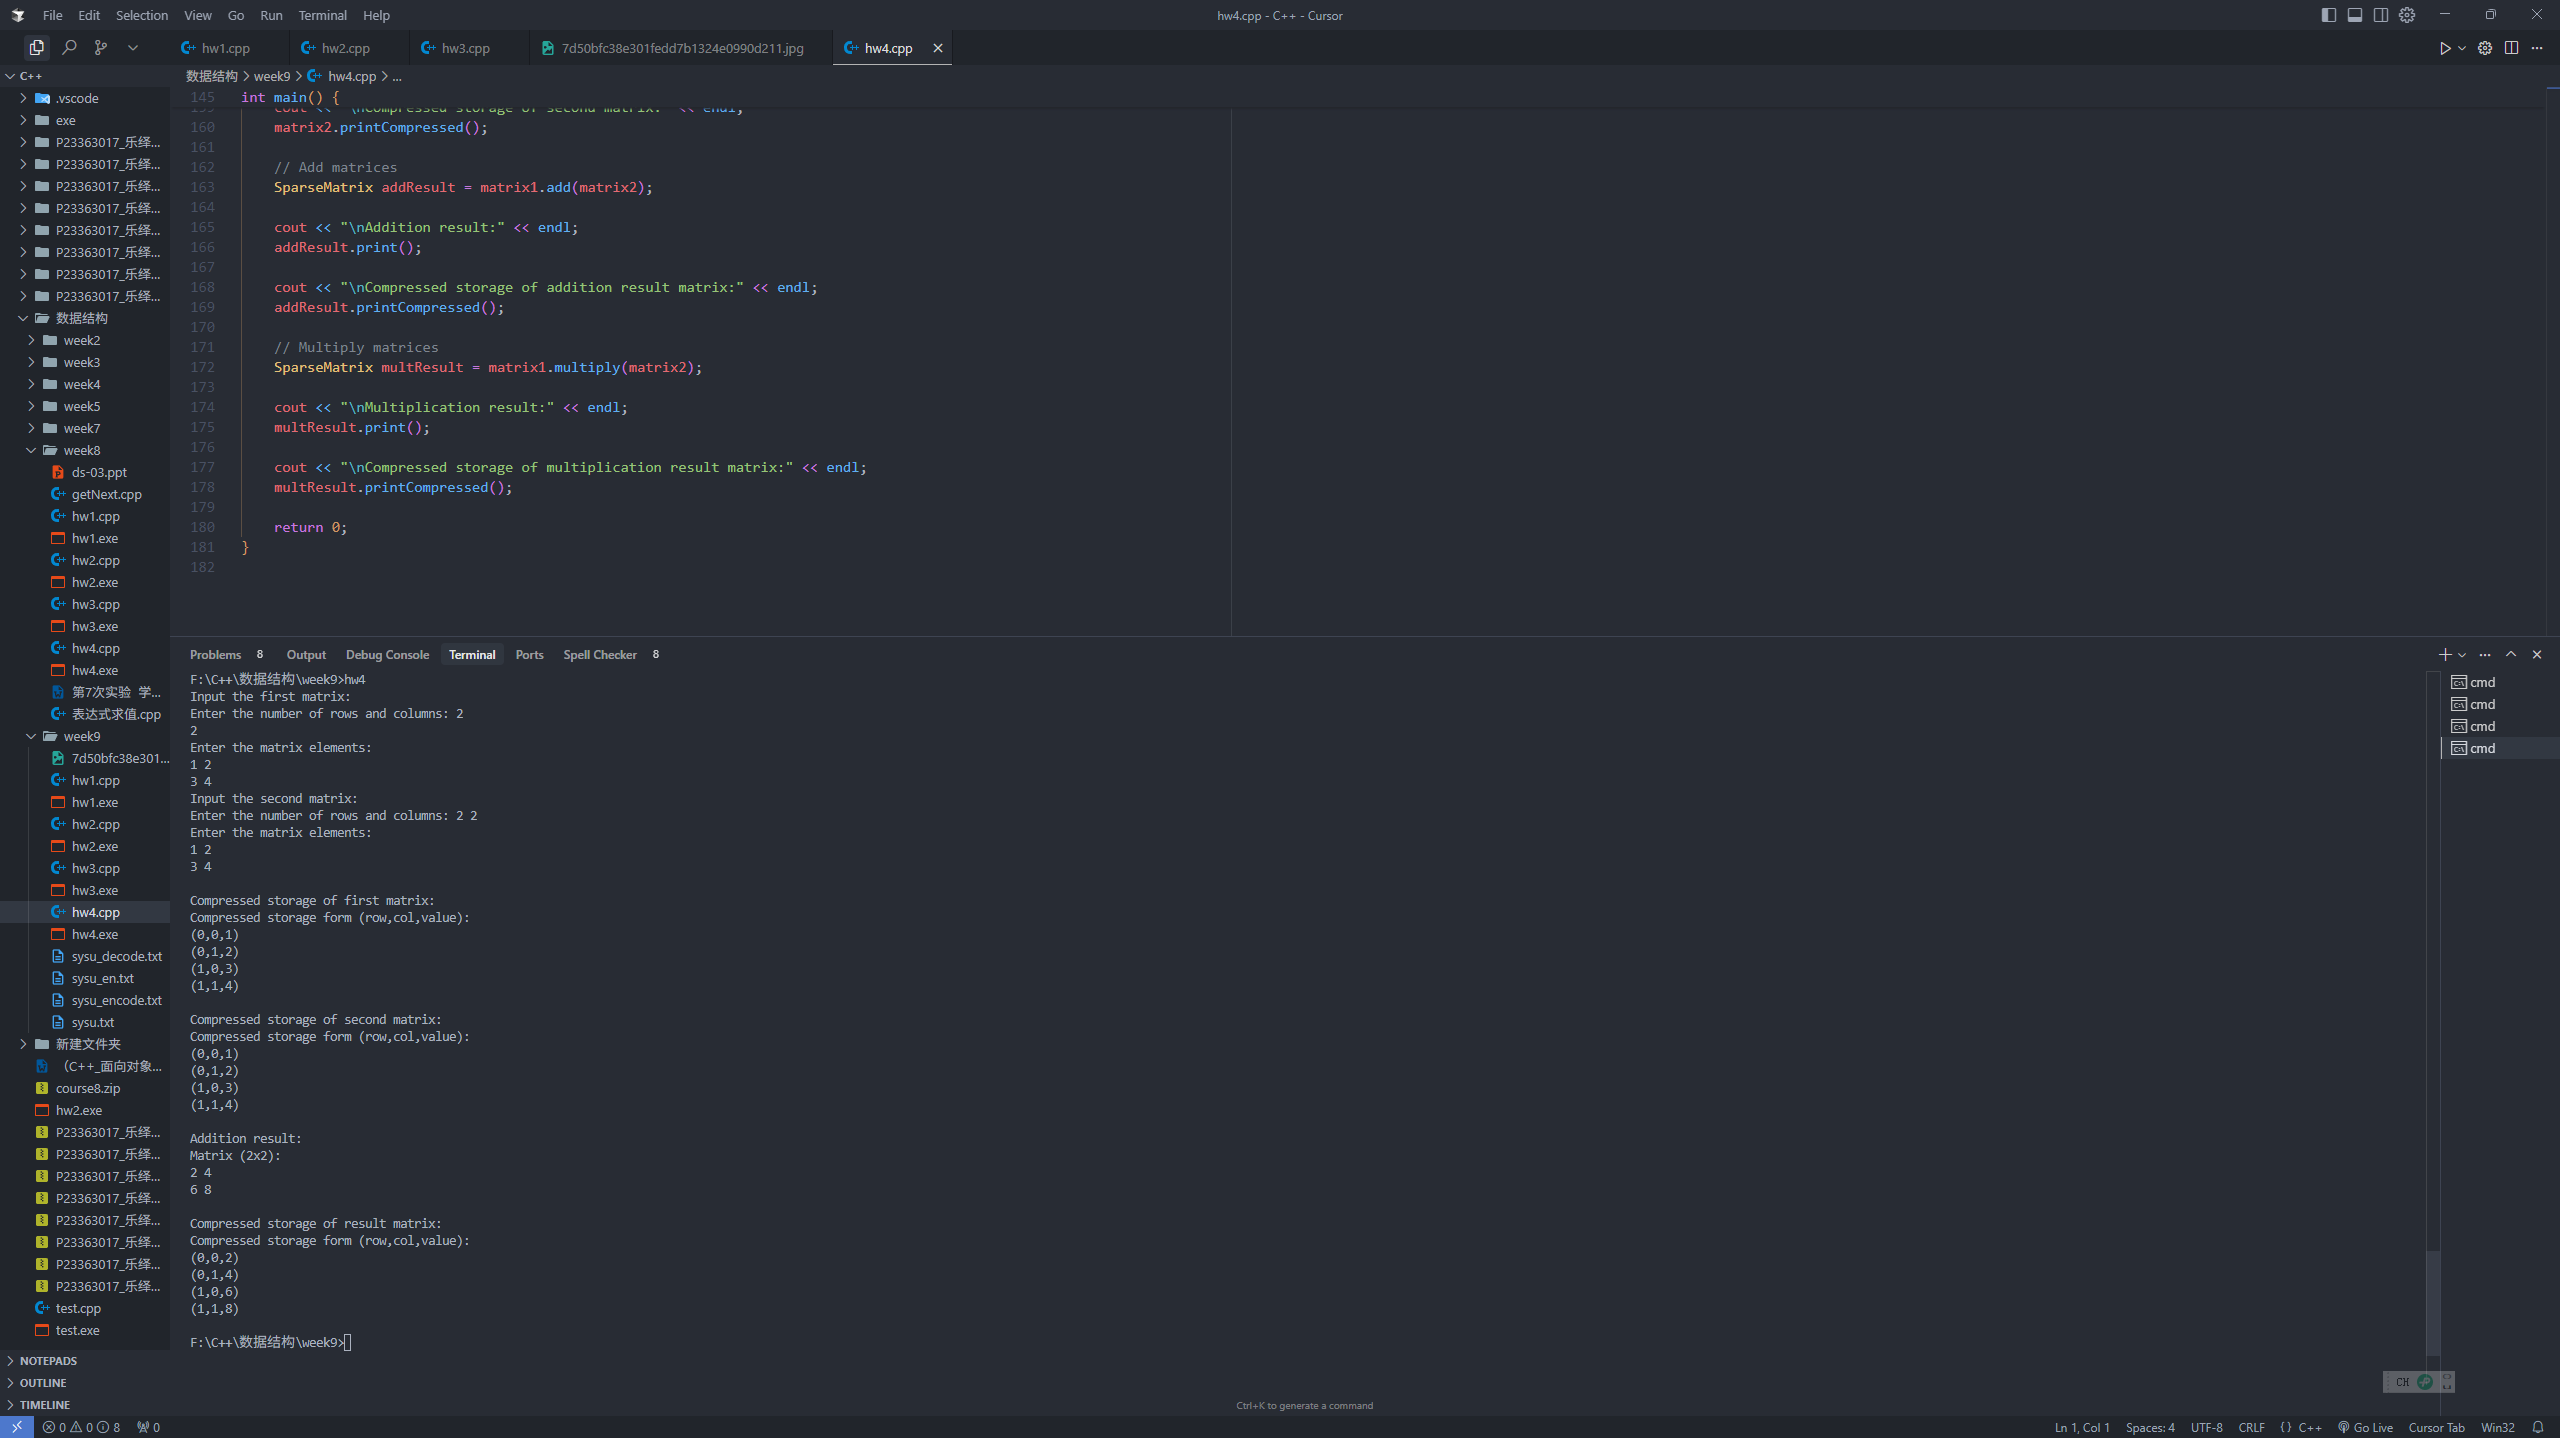
\includegraphics[width=\textwidth]{1-实验报告8-2025042823.png}
% \caption{}
\label{}
\end{figure}

\begin{lstlisting}[language=C++]
#include <iostream>

#include <vector>

using namespace std;

  

// Triple structure to represent non-zero elements

struct Triple {

    int row, col, value;

};

  

// Sparse Matrix class

class SparseMatrix {

private:

    int rows, cols;

    vector<Triple> data;

  

public:

    // Constructor

    SparseMatrix(int r, int c) : rows(r), cols(c) {}

  

    // Add a non-zero element

    void addElement(int r, int c, int val) {

        if (val != 0) {

            data.push_back({r, c, val});

        }

    }

  

    // Read matrix from user input

    void readFromInput() {

        cout << "Enter the number of rows and columns: ";

        cin >> rows >> cols;

        cout << "Enter the matrix elements:" << endl;

        for (int i = 0; i < rows; i++) {

            for (int j = 0; j < cols; j++) {

                int val;

                cin >> val;

                if (val != 0) {

                    addElement(i, j, val);

                }

            }

        }

    }

  

    // Print the sparse matrix (full form)

    void print() const {

        vector<vector<int>> fullMatrix(rows, vector<int>(cols, 0));

        // Fill in non-zero elements

        for (const auto& t : data) {

            fullMatrix[t.row][t.col] = t.value;

        }

        // Print the complete matrix

        cout << "Matrix (" << rows << "x" << cols << "):" << endl;

        for (int i = 0; i < rows; i++) {

            for (int j = 0; j < cols; j++) {

                cout << fullMatrix[i][j] << " ";

            }

            cout << endl;

        }

    }

  

    // Print compressed storage form

    void printCompressed() const {

        cout << "Compressed storage form (row,col,value):" << endl;

        for (const auto& t : data) {

            cout << "(" << t.row << "," << t.col << "," << t.value << ")" << endl;

        }

    }

  

    // Matrix addition

    SparseMatrix add(const SparseMatrix& other) const {

        if (rows != other.rows || cols != other.cols) {

            cerr << "Matrix dimensions don't match, cannot add!" << endl;

            return SparseMatrix(0, 0);

        }

  

        SparseMatrix result(rows, cols);

        // Create full representation of result matrix

        vector<vector<int>> resultMatrix(rows, vector<int>(cols, 0));

        // Add elements from first matrix

        for (const auto& t : data) {

            resultMatrix[t.row][t.col] += t.value;

        }

        // Add elements from second matrix

        for (const auto& t : other.data) {

            resultMatrix[t.row][t.col] += t.value;

        }

        // Add non-zero elements to result matrix

        for (int i = 0; i < rows; i++) {

            for (int j = 0; j < cols; j++) {

                if (resultMatrix[i][j] != 0) {

                    result.addElement(i, j, resultMatrix[i][j]);

                }

            }

        }

        return result;

    }

    // Matrix multiplication

    SparseMatrix multiply(const SparseMatrix& other) const {

        if (cols != other.rows) {

            cerr << "Matrix dimensions don't match, cannot multiply!" << endl;

            return SparseMatrix(0, 0);

        }

        SparseMatrix result(rows, other.cols);

        // Create full representation of result matrix

        vector<vector<int>> resultMatrix(rows, vector<int>(other.cols, 0));

        // Convert sparse matrices to full matrices for multiplication

        vector<vector<int>> mat1(rows, vector<int>(cols, 0));

        vector<vector<int>> mat2(other.rows, vector<int>(other.cols, 0));

        for (const auto& t : data) {

            mat1[t.row][t.col] = t.value;

        }

        for (const auto& t : other.data) {

            mat2[t.row][t.col] = t.value;

        }

        // Perform matrix multiplication

        for (int i = 0; i < rows; i++) {

            for (int j = 0; j < other.cols; j++) {

                for (int k = 0; k < cols; k++) {

                    resultMatrix[i][j] += mat1[i][k] * mat2[k][j];

                }

                if (resultMatrix[i][j] != 0) {

                    result.addElement(i, j, resultMatrix[i][j]);

                }

            }

        }

        return result;

    }

};

  

int main() {

    // Create two sparse matrices

    SparseMatrix matrix1(0, 0);

    SparseMatrix matrix2(0, 0);

    cout << "Input the first matrix:" << endl;

    matrix1.readFromInput();

    cout << "Input the second matrix:" << endl;

    matrix2.readFromInput();

    cout << "\nCompressed storage of first matrix:" << endl;

    matrix1.printCompressed();

    cout << "\nCompressed storage of second matrix:" << endl;

    matrix2.printCompressed();

    // Add matrices

    SparseMatrix addResult = matrix1.add(matrix2);

    cout << "\nAddition result:" << endl;

    addResult.print();

    cout << "\nCompressed storage of addition result matrix:" << endl;

    addResult.printCompressed();

    // Multiply matrices

    SparseMatrix multResult = matrix1.multiply(matrix2);

    cout << "\nMultiplication result:" << endl;

    multResult.print();

    cout << "\nCompressed storage of multiplication result matrix:" << endl;

    multResult.printCompressed();

    return 0;

}
\end{lstlisting}